\paragraph{Development accepted-set accounting.}
Direct excess gains 6.08 percentage points in mean row coverage over forecast-normalized error, but loses 5.71 points of demand coverage. At the first seed, their common accepted set covers 73.35\% of rows and has WAPE 0.5958, leaving slack under the 0.64013 cap. The direct-only set adds 267,656 rows (12.84\% of all rows), but only 5.69\% of demand; its WAPE is 1.0026. The relative-only set contains 141,617 rows and 11.45\% of demand, with WAPE 0.7915. Mean forecasts in the two differing sets are 0.039 and 1.498 units. In equation~\eqref{eq:budget}, the common set supplies 97,185.97 units of excess slack. The direct-only set consumes 60,141.11 (61.88\%), versus 50,549.56 (52.01\%) for the relative-only set. Both fit within the pooled budget despite their individual WAPE exceeding the cap. This accounts for the row gain through budget use and demand composition.


\paragraph{Architecture is distinct from acceptance utility.}
The original matched selector comparison provides an architectural control. Direct-excess, two-head, and matched-tree-budget two-head scores reach 86.30\%, 86.35\%, and 86.61\% mean row coverage. Direct learning has slightly lower accepted WAPE (0.6245 versus 0.6268 and 0.6269); it does not establish a direct-learning advantage. The informative distinction is the coverage objective and resulting budget allocation, not whether excess is learned directly or composed from two heads. Full three-seed results are in Appendix~\ref{app:objective}.

\subsection{Detailed first item-holdout comparison}
\label{app:architecture-holdout}
\begin{table}[t]
\centering\small
\caption{Previously held-out M5 items: fixed pooled thresholds, 610 items, 6,100 series, and 695,400 shadow rows. Three-seed means; all fits and thresholds were frozen before opening. Seeds measure training variability, not three independent holdouts. Absolute-error selection accepts no rows and has undefined WAPE.}
\label{tab:m5guardian}
\begin{tabular}{lrrr}\toprule
Score & Row coverage (\%) & Demand coverage (\%) & WAPE\\\midrule
Forecast-normalized & 80.87 & 87.65 & 0.6219 \\
Demand-normalized & 73.62 & 88.23 & 0.6219 \\
Forecast excess & 82.74 & 74.59 & 0.6251 \\
Two-head excess (440) & 87.41 & 83.69 & 0.6297 \\
Two-head excess (220) & 87.67 & 84.18 & 0.6297 \\
Direct excess (220) & 87.37 & 83.29 & 0.6280 \\
\bottomrule\end{tabular}
\end{table}

The freeze specifies seven scores, two threshold modes, three seeds, and a first-seed direct-versus-two-head primary contrast. The holdout uses the same A/B and later evaluation dates, without recalibration; no holdout outcome selects an original policy. Its shadow contains 695,400 rows on days 1800--1913.

The coverage trade-off persists (Table~\ref{tab:m5guardian}). Across three fixed fits, direct excess increases row coverage by 6.49 percentage points over forecast-normalized error while reducing demand coverage by 4.36 points. Two-head coverage is 87.41\%, compared with 87.37\% for direct learning, with WAPE 0.6297 versus 0.6280. At the prespecified first seed, direct minus two-head row coverage is $-0.215$ points (paired 95\% item-bootstrap interval $[-0.413,-0.018]$ points); direct WAPE is lower by 0.00141. These are different trade-offs, not an equivalence result or a direct-learning advantage.



Operating constraints do not transfer jointly. First-seed direct and two-head shadow WAPE are 0.6282 and 0.6296 pooled, but approximately 0.879 for Hobbies and 0.682--0.683 for Household. In the holdout window matching calibration B, even pooled WAPE is 0.6495 and 0.6504, above the 0.64013 cap. All frozen category-specific policies abstain entirely on Hobbies because their development threshold is absent. The prespecified 48-endpoint family covers two primary methods, three periods, four strata, and two bounds, using 10,000 item-bootstrap draws. Every coverage lower bound exceeds 0.35, but every adjusted WAPE upper bound exceeds the cap; shadow pooled upper bounds are 0.6959 and 0.6971. This fails the specified joint operating check. Appendix~\ref{app:heldout} reports all bounds and the access record.


\begin{figure}[t]
\centering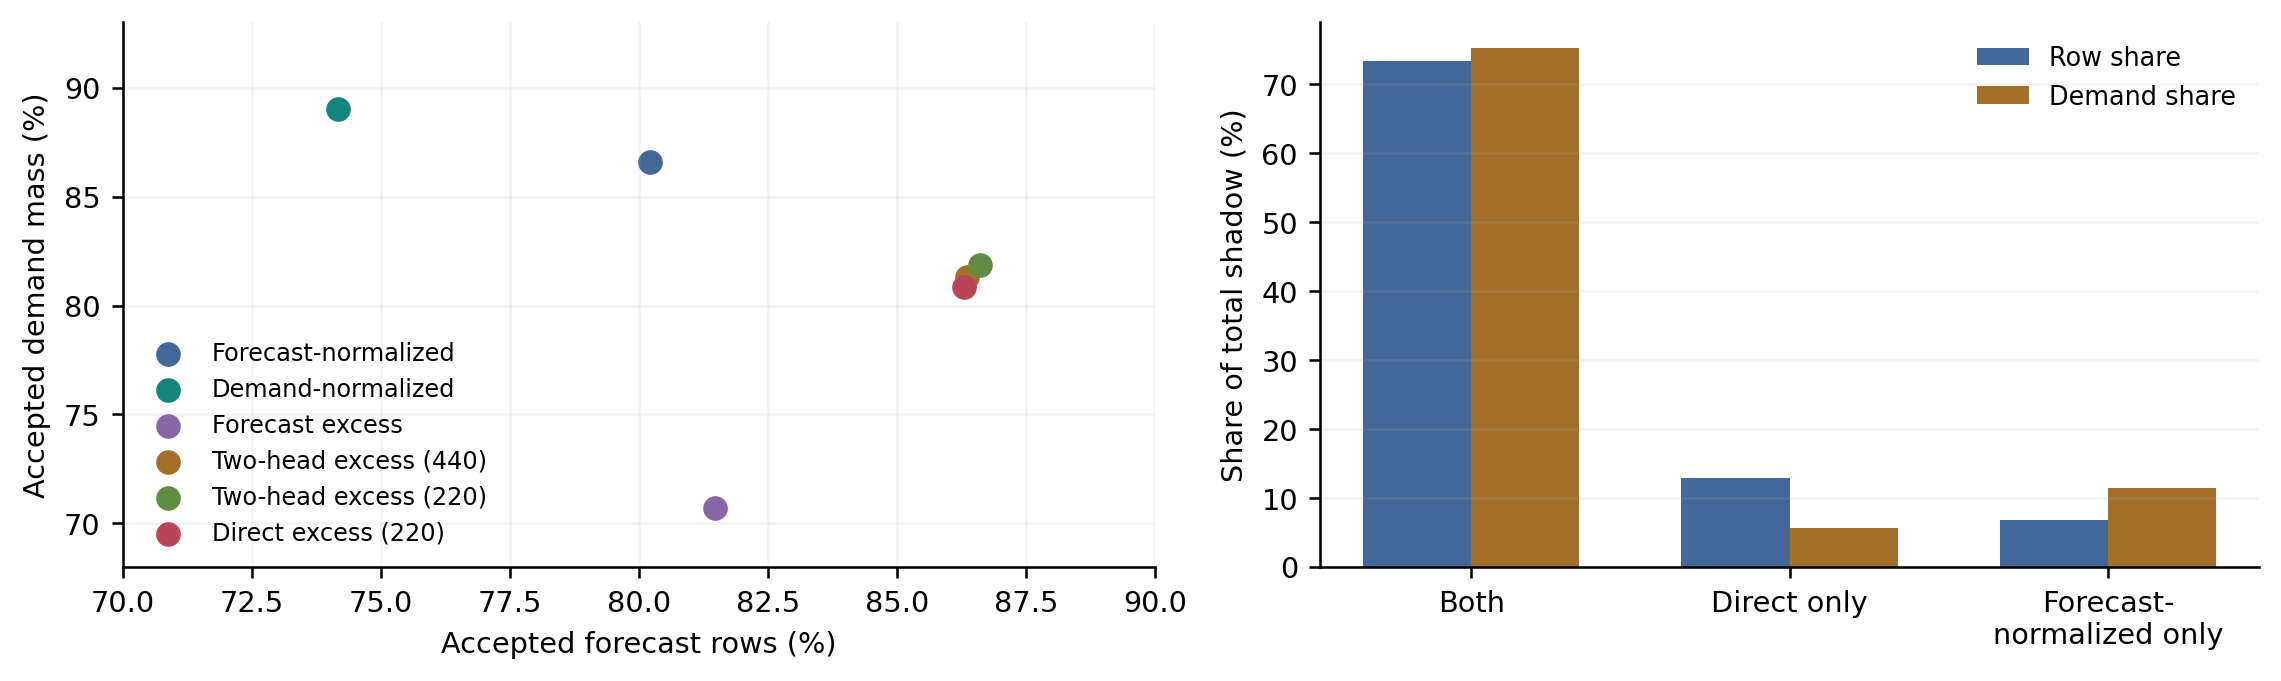
\includegraphics[width=\linewidth]{figures/row_vs_demand.png}
\caption{Original development comparison. Left: three-seed means under row-coverage threshold selection. Right: first-seed direct-excess and forecast-normalized-error acceptance sets. The direct-only set has more cases and less demand. These previously evaluated results precede the additional menu audit.}
\label{fig:mass}
\end{figure}
